% !TeX root = ../main-english.tex
% !TeX spellcheck = en-US
% !TeX encoding = utf8
% -*- coding:utf-8 mod:LaTeX -*-

%This smart spell only works if no changes have been made to the chapter
%using the options proposed in preambel/chapterheads.tex.
\setchapterpreamble[u]{%
	\dictum[Albert Einstein]{We cannot solve our problems with the same level of thinking that created them}
}
\chapter{Introduction}
\label{chap:k1}

Look mom, some text!

\section{Brain state spaces}
This is an introduction into brain states and functional alignment
\pagebreak

\section{Magnetoencephalograpy (MEG)}
This is an introduction into \gls{meg} data
\pagebreak

\section{Research data management}
%This is an introduction on the importance of research data management for reproducible science

Research data encompasses everything that is produced in the life span of a research project.
This could include raw data acquisitions, preprocessed or otherwise standardized datasets, software, analysis scripts, results, compiled reports or articles, figures, tables, and many other final or intermediate outcomes of a research process.
To disambiguate ``research data'' from the smaller-scoped meaning that terms such as ``data'' or ``dataset'' carry in colloquial language (for example, the outcome of a data acquisition in an experiment), it is also referred to in the literature as ``research objects``, and, in case it exists in purely electronic form, as ``digital research objects''. (CITATION NEEDED)
\gls{rdm} describes the handling of these research objects through their entire life cycle: from curation, use, publication and sharing, archiving to re-use or destruction \ref{fig:rdm-lifecycle}.

\begin{figure}
	\centering
	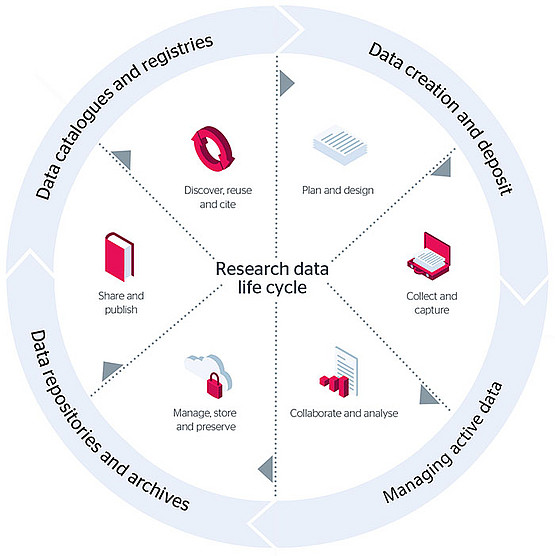
\includegraphics[width=.5\textwidth]{rdm-lifecycle-jisc.png}
	\caption[The life cycle of digital research objects]{The life cycle of digital research objects. License: JISC Research data management toolkit (\href{https://www.jisc.ac.uk/guides/rdm-toolkit}{www.jisc.ac.uk/guides/rdm-toolkit}), CC-BY-ND}
	\label{fig:rdm-lifecycle}
\end{figure}

Typically, research objects have a much longer life span than the project that creates them.
Research data management ensures that research objects are preserved to act as an evidence base for findings and as a resource for further reuse.
As such, \gls{rdm} is a foundational element within good scientific practice, and, as I will lay out in this section and in upcoming chapters, an important prerequisite for computational modeling.


\subsection{The FAIR guiding principles for scientific data management and stewardship}

Since their publication, the so-called \glsunset{FAIR}\gls{FAIR} principles \citep{wilkinson2016fair} have become guidelines for \gls{rdm} efforts for digital research objects.
They describe four measurable properties of research data that -- the better they are fulfilled -- serve the ultimate goal to improve the discoverability and reusability of data by machines and humans alike \citep{wilkinson2016fair}.
The \gls{FAIR}ness of data can be improved on each of the four related but separable major characteristics that are behind the \gls{FAIR} acronym (taken verbatim from \citet{wilkinson2016fair}):

\begin{itemize}
	\item \textbf{F}indable: To be Findable, (meta)data  are assigned a globally unique and persistent identifier (F1); data are described with rich metadata (F2); metadata clearly and explicitly include the identifier of the data it describes (F3);  (meta)data are registered or indexed in a searchable resource (F4)
	\item \textbf{A}ccessible: To be Accessible, (meta)data are retrievable by their identifier using a standardized communications protocol (A1); the protocol is open, free, and universally implementable (A1.1); the protocol allows for an authentication and authorization procedure, where necessary (A1.2);  metadata are accessible, even when the data are no longer available (A2)
	\item \textbf{I}nteroperable:  To be Interoperable, (meta)data use a formal, accessible, shared, and broadly applicable language for knowledge representation (I1); (meta)data use vocabularies that follow FAIR principles (I2); (meta)data include qualified references to other (meta)data (I3); and
	\item \textbf{R}eusable: To be Reusable, meta(data) are richly described with a plurality of accurate and relevant attributes (R1); (meta)data are released with a clear and accessible data usage license (R1.1); (meta)data are associated with detailed provenance (R1.2); (meta)data meet domain-relevant community standards (R1.3)
\end{itemize}

The ``term machine-actionable'' is central to the \gls{FAIR} principles, and is used to describe a ``continuum of possible states wherein a digital object provides increasingly more detailed information to an autonomously-acting, computational data explorer'' \citep{wilkinson2016fair}.
% add metadata


Importantly, the \gls{FAIR} principles do not suggest specific metadata standards, implementations, or technology choices.
The following sections will outline \gls{rdm} requirements and solutions in the field of neuroimaging, and the end of this chapter is dedicated to  highlight one of several software tools that aids with the complex tool of research data management: DataLad.

\subsection{Research data management in neuroimaging}
\label{chap:k1-rdm-2}

The following section contains a subset of the work presented in our original publication \citet{NISO2022119623}.

The field of neuroimaging is characterized by complex datasets, typically encompassing different modalities (such as imaging, electro-physiological, and behavioral measurements) and often several recording sessions.
The processing of neuroimaging data usually entails multi-stepped workflows from acquisition through analysis to archival which often involve several software tools at every step \citep{poline2011}.
The \gls{BIDS} \citep{gorgolewski2016brain} is a community standard for organizing and describing neuroimaging data, and is widely considered as a successful solution for data standardization in such datasets.
It defines common and modality specific schemes for file names and file organization, file formats, and metadata to accompany raw or derived data.
\gls{BIDS} has widespread and growing support for different neuroimaging modalities, and is made a common prerequisite by neuroscientific data portals such as OpenNeuro \citep{markiewicz2021openneuro} or processing tools such as BIDSApps \citep{gorgolewski2017bids}.


% add more on RDM

Additionally, the growing awareness of the role of sample size for robust results \citep{button2013power} \citep{turner2018small} and a focus on diverse, representative samples has resulted in datasets of unprecedented size.
In the neurosciences, datasets scale to millions of files, hundreds of terabytes6,7, acquired from tens of thousands of participants. Well known examples, such as the Human Connectome Project8, the Adolescent Brain Cognitive Development Study (ABCD)9, or the UK Biobank (UKB) project10, contain diverse data ranging from brain imaging to genetics to clinical and non-clinical measures.

This chapter will further showcase how research data management is a foundational element of reproducible research.
research data management is a foundational element of reproducibility \citep{borghi2021promoting}


The following section will  highlight one of several software tools that aids with the complex tool of research data management: DataLad. The following \cref{chap:k1} will outline how software usability can improve scientific practice, using DataLad and its user-facing documentation, the DataLad Handbook, as an example.
The upcoming \cref{chap:k2} will then focus specifically on two aspects of research data management for reproducibility: Software environments, and scalability to large sample sizes.
In addition, \cref{chap:k2} will highlight pragmatic approaches to \gls{rdm} that can be embedded in standard research practice and contribute to the FAIRification of data, even in absence of established metadata formats.


% What is research data management
%% FAIR

% Why is it important
%% Reproducibility crisis


% What can we do to improve research data management
%% BIDS, read Niso paper

The building blocks of scientific results extend to more than the files that constitute the actual research output, but also to all elements involved in its generation \citep{claerbout1992electronic}.
Consider three types of research output: Raw data originates from acquisitions based on - potentially ongoing - experiments, raw data transformations, or data cleaning, processed data or results stem from computations with analysis code or software in specific versions on particular data, and software, expressed in raw (code) or derived (transformed into executable) form, is created or used in specific computational environments, with compilers, underlying libraries, and systems in distinct versions.
Those building blocks are integral information to retrace the genesis, reproduce, or trust research outputs (Kennedy et al., 2019), but they are rarely ever static.
Whatever created a given output evolves during usually incremental processes such as continuous quality control, acquisition, maintenance, or project revision.
However, changes in these building blocks will influence the resulting research output \citep{kennedy2019everything} 2019),\citep{glatard2015reproducibility}.
If it is not possible to precisely identify the foundational elements and everything involved in their creation, the reproducibility and reusability of research outputs and projects that use these objects is hence threatened \citep{kennedy2019everything}.

% provenance
\begin{figure}
	\centering
	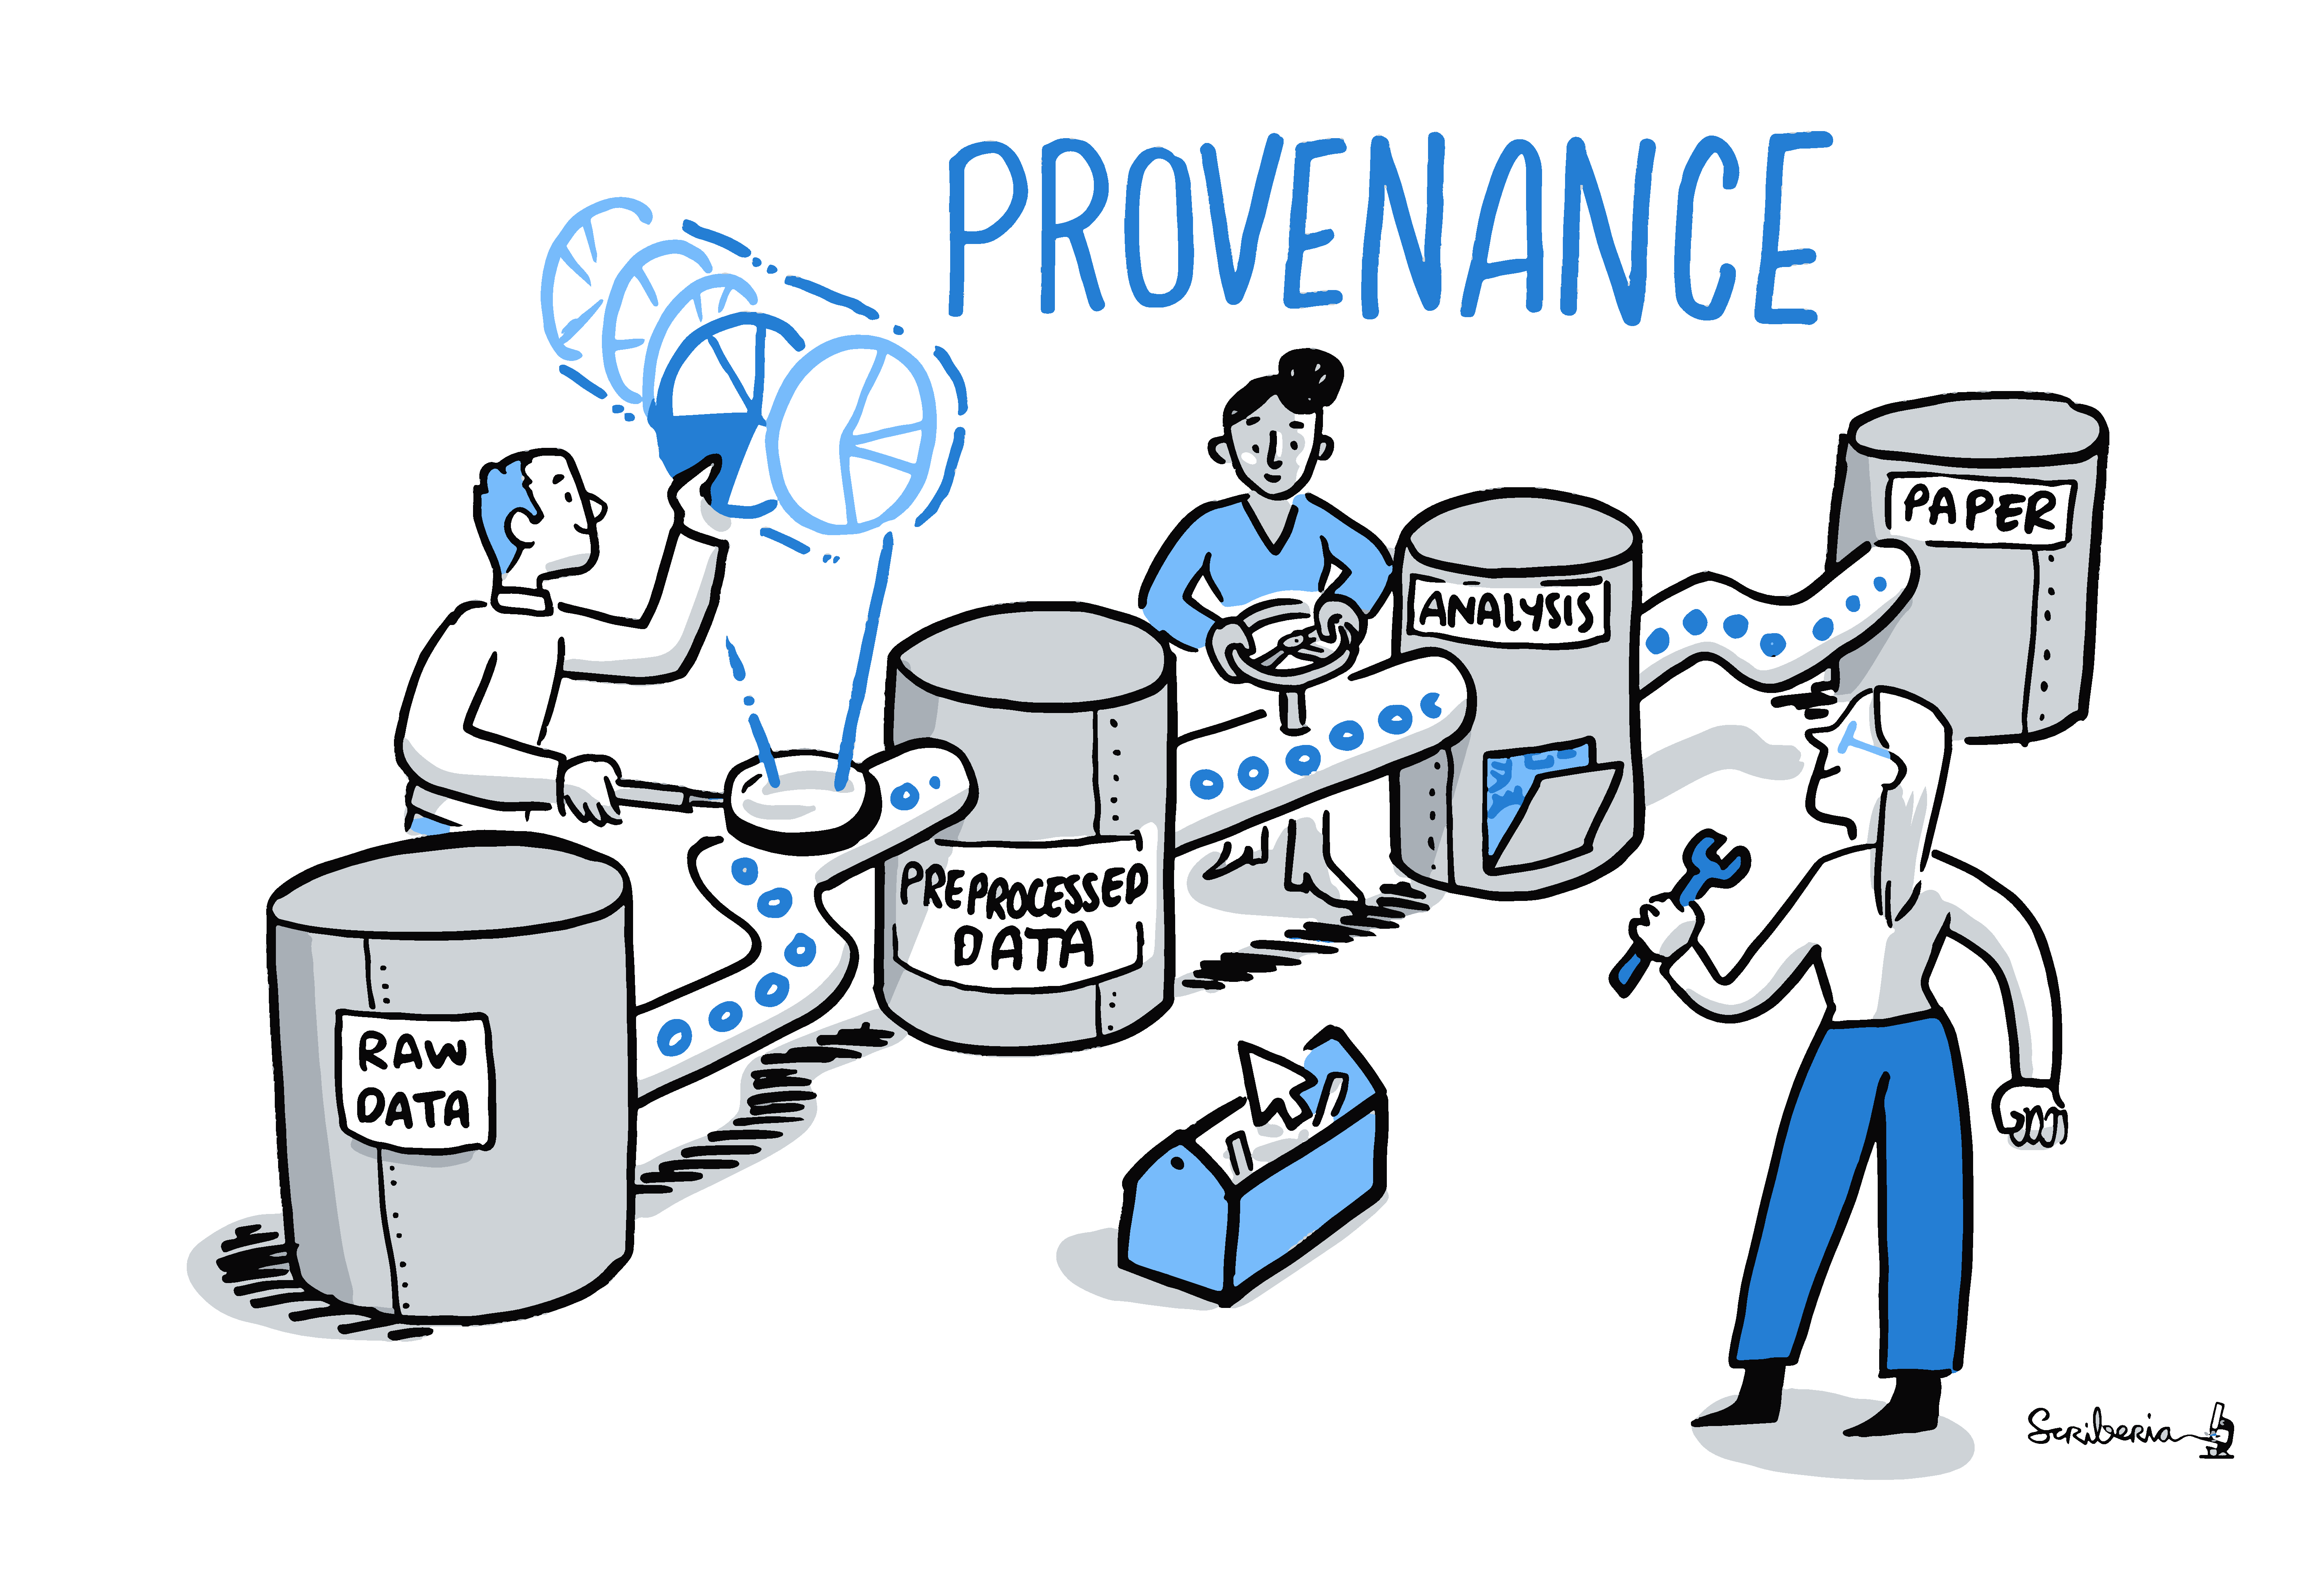
\includegraphics[width=\textwidth]{provenance.pdf}
	\caption[Software provenance throughout the research process]{License: Scriberia and the Turing Way Project, CC-BY}
	\label{fig:prov1}
\end{figure}


% link to chapter 3: Research data management is a prerequisite of reproducible research

\pagebreak

\section{DataLad as a software solution for research data management challenges}

The following section provides an overview of the features of the software tool DataLad and their use for research data management.
The reader is invited to refer to our original publications \citep{Halchenko2021} \citep{wagner2020datalad} for a more detailed description.
%This introduces DataLad as a software solution for research data management

\subsection{An overview of features and their use for \gls{rdm}}

Although many solutions to common challenges exist, putting \gls{rdm} into practice remains a complicated endeavor:
In most neuroimaging studies, scientific insights are created from well-described raw data and its derivatives.
Standards and repositories as mentioned in \cref{chap:k1-rdm-2} form a basis for managing, storing and sharing them, and being able to efficiently retrieve and update these research objects across a variety of available storage options is an important part of \gls{rdm} \citep{borghi2018data}.
However, homogeneous data transport is complicated by disconnected and non-interoperable hosting solutions.
Different storage services can require different protocols, means of authentication, or other idiosyncrasies (CITATION NEEDED). \\
Over the course of a research project, often as part of the standard, multi-stepped processing workflow \citep{poline2011}, data also evolve and change:
Continued acquisitions enlarge the raw dataset.
Transformations to community standards such as \gls{BIDS} \citep{gorgolewski2016brain} change file formats, dataset organization, or enrich available metadata.
Continuous quality control processes or accidental findings can bring errors to light and improve datasets with fixes (e.g., CITATION NEEDED).
In the case that data or other research objects were subject to change over the course of a project, there is a need to identify which exact version has been used -- otherwise, the reproducibility of a result is threatened (CITATION NEEDED). \\
Likewise, projects might draw insights from only a subset of a dataset, such as only specific modalities, tasks, or participants, despite much greater data availability.
If the original dataset, however, is only available as a bulk download, a project has heavier disk space demands on storage solutions than their eventual data requirements.
Especially in the age of big data neuroscience \citep{bzdok2017inference}, downloads or storage of standard large-scale datasets can become infeasible \citep{horien2021hitchhiker} \citep{grisham2016proposed}. \\
Finally, \textit{digital provenance}, the information bout how tools, data, and actors were involved in the generation of a digital research outcome is crucial to understand and reproduce a result, but rarely fully transparent and documented, let alone machine-readable or actionable.
% NISO The ability to manage data and metadata and track the data-analysis process provides a basis for rigor and reproducibility.


DataLad (\href{http://datalad.org}{datalad.org}) \citep{Halchenko2021} is a Python-based, MIT-licensed software tool for the joint management of code, data, and their relationship, developed with the aim to assist with common \gls{rdm} tasks in science.
Its main features provide solutions to the difficulties outlined above:
Building up on established open source version control tools, Git (CITATION) and git-annex (CITATION NEEDED), DataLad provides the ability to version control data of any size or type.
Bridging a large variety of storage and Git repository hosting services with its interoperability layer, it streamlines procedures to consume, publish, and update digital data, and unifies authentication procedures for an end user.
Due to a separation between file content and file identity metadata, DataLad allows
- fine grained access control for data providers
- downloads at single file granularity for data users
- lightweight but actionable access to data

With dedicated functionality to capture complete and actionable process provenance of data transformations and allow automatic re-computation, DataLad can record machine-actionable metadata how files came into existence.
Based on Git's submodule mechanism, DataLad allows for modular structuring of ...
 for  and to link them as precisely versioned, lightweight
dependencies. DataLad helps to make science more reproducible and FAIR (Wilkinson et al.,
2016). It can capture complete and actionable process provenance of data transformations to
enable automatic re-computation.

Fundamental to DataLad's functionality is the concept of the ``DataLad dataset'', DataLad's central data structure.
On a technical level, it is a joint Git/git-annex repository.

%% from datalad paper:


Code, data and computing environments are core components of scientific projects. While
the collaborative development and use of research software and code is streamlined with es-
tablished procedures and infrastructures, such as software distributions, distributed version
control systems, and social coding portals like GitHub, other components of scientific projects
are not as transparently managed or accessible. Data consumption is complicated by discon-
nected data portals that require a large variety of different data access and authentication
methods. Compared with code in software development, data tend not to be as precisely
identified because data versioning is rarely or only coarsely practiced. Scientific computation
is not reproducible enough, because data provenance, the information of how a digital file
came to be, is often incomplete and rarely automatically captured. Last but not least, in
the absence of standardized data packages, there is no uniform way to declare actionable
data dependencies and derivative relationships between inputs and outputs of a computa-
tion. DataLad aims to solve these issues by providing streamlined, transparent management
of code, data, computing environments, and their relationship. It provides targeted interfaces
and interoperability adapters to established scientific and commercial tools and services to
set up unobstructed, unified access to all elements of scientific projects. This unique set of
features enables workflows that are particularly suited for reproducible science, such as ac-
tionable process provenance capture for arbitrary command execution that affords automatic
re-execution. To this end, it builds on and extends two established tools for version control
and transport logistics, Git and git-annex.


\subsection{Software adoption and relevance}

DataLad does not employ tracking code.
As such, the exact number of its users is not known.
However, download statistics from the major Python package managers \texttt{pip} and \texttt{conda}, and popularity statistics from users of the Debian operating system can provide rough references.
According to pypistats.org, the main DataLad Python package was downloaded from the Python Package Index 300 times per day on average in May 2023.
The Python distribution Anaconda (anaconda.org) counts a total of 333932 downloads of the software throughout versions 0.9.3 (April 2018) and 0.18.3 (May 2023), averaging 180 downloads per day.
The \texttt{popularity-contest} software is a Debian package that, if installed on a users system, reports anonymous statistics about most-used Debian packages.
This data is aggregated into a popularity contest.
According to it, in May 2023 between 0.04 and 0.05 percent of systems reporting statistics have an installation of the DataLad Debian package, or the equivalent python3-datalad Debian package.
All of these sources contain biases that limit conclusion to the number of users, though.
Installations via Python package managers are commonly performed by individual end users, whereas installations of Debian packages can correspond to system-wide installations on multi-user systems such as high performance computing infrastructure.
Likewise, upgrades of existing installations to more recent versions are included in these data, as well as temporary installations of the software in automated continuous integration test suites.
Nevertheless, download statistics confirm that it is an actively used tool with a user base that exceeds the circle of its developers by far.
This is also confirmed by citations of the academic paper, totaling 51 1.5 years after its publication by \citet{Halchenko2021}, and active contributor community around the source repository on GitHub, currently amounting to 48 individuals with committed code contributions.



\pagebreak

